\subsection{Сітки і сіткові функції}

\subsubsection{Сітки}

\begin{enumerate}
    \item Одновимірна рівномірна сітка: задана область $\bar \Omega = [a, b]$, її границя $\partial \bar \Omega = \Gamma$. Власне сітки:
    \begin{align}
        \label{eq:4.2.1}
        \bar \omega_h &= \{x_i = a + i h, h = (b - a) / N, i = \overline{0, N}\}, \\
        \label{eq:4.2.2}
        \omega_h &= \{x_i = a + i h, h = (b - a) / N, i = \overline{1, N - 1}\},
    \end{align}
    де $\gamma_h = \bar \omega_h \setminus \omega_h = \{a, b\}$ --- вузли на границі.
    
    \item Нерівномірна сітка: там сама область, але
    \begin{equation}
        \label{eq:4.2.3}
        \bar \omega = \{ x_i = x_{i - 1} + h_i, \sum_{i = 1}^n h_i = b - a \} ,
    \end{equation}
    де $\gamma_h = \{x_0 = a, x_n = b\}$ --- вузли на границі.
    
    \item Просторово-часова сітка: задана область $\bar Q_T = \Omega \times [0, T]$, її границя $\partial Q_T = \partial \Omega \times (0, T)$. Власне сітка:
    \begin{equation}
        \label{eq:4.2.4}
        \bar \omega_{h, \tau} = \bar \omega_h \times \bar \omega_\tau,
    \end{equation}
    де
    \begin{align}
        \label{eq:4.2.5}
        \bar \omega_h &= \{ x_i = a + i h, i = \overline{0, N}, h = (b - a) / N\}, \\
        \label{eq:4.2.6}
        \bar \omega_\tau &= \{ t_i = j \tau, j = \overline{0, M}, \tau = T / M\}.
    \end{align}
    
    \item Двовимірна сітка: задана область $\bar \Omega = \bar \Omega_1 \times \bar \Omega_2$, де $\Omega_1 = [a, b]$, і $\Omega_2 = [c, d]$. Власне сітка:
    \begin{equation}
        \label{eq:4.2.7}
        \bar \omega_{h_1, h_2} = \bar \omega_{h_1} \times \bar \omega_{h_2},
    \end{equation}
    де
    \begin{align}
        \label{eq:4.2.8}
        \bar \omega_{h_1} &= \{ x_i = a + i h_1, i = \overline{0, N}, h_1 = (b - a) / N\}, \\
        \label{eq:4.2.9}
        \bar \omega_{h_2} &= \{ y_j = c + j h_2, i = \overline{0, M}, h_2 = (d - c) / M\}.
    \end{align}
    
    \item $\Omega$ --- довільна область у двовимірній площині. Власне сітка:
    \begin{equation}
        \label{eq:4.2.10}
        R_{h_\alpha} = \{x_{\alpha_i} = i h, i = 0, \pm 1, \pm 2, \ldots, \alpha = 1, 2\},
    \end{equation}
    де
    \begin{equation}
        \label{eq:4.2.11}
        R_h = R_{h_1} \times R_{h_2}, \quad \omega_h = R_h \cap \Omega.
    \end{equation}
\end{enumerate}

\subsubsection{Сіткові функції}

\begin{enumerate}
    \item Розглянемо простір $B_1 = C([a, b])$, норма у якому визначається як $\|u\|_C = \max_{a \le x \le b} |u(x)|$. Тоді простір
    $B_{1,h} = C(\bar \omega_h)$, і у ньому норма вже $\|y\|_{C(\omega_h)} = \max_{\omega_h} |y_i|$.

    \item Розглянемо (гільбертів) простір $B_1 = H = L_2([a, b])$, норма у якому визначається як $\|u\|^2 = \int_a^b u^2 \diff x$. Тоді простір $B_{1,h} = L_2(\omega_h)$, і у ньому норма вже
    \begin{equation}
        \label{eq:4.2.12}
        \|y\|_{L_2(\omega_h)} = h \sum_{i = 1}^{N - 1} y_i^2 + \frac{h}{2} (y_0^2 + y_N^2).
    \end{equation}
    \stepcounter{equation}
    
    По суті нова норма --- початковий інтеграл, записаний через формулу трапецій. До речі, проектування для цієї пари просторів матиме вигляд
    \begin{equation}
        \label{eq:4.2.14}
        P_{1,h}(u) = \begin{cases}
            \dfrac{2}{h} \Int_{x_0}^{x_0 + h/2} u(x) \diff x, & x = x_0, \\[.5ex]
            \dfrac{1}{h} \Int_{x_{i - 1/2}}^{x_{i + 1/2}} u(x) \diff x, & x = x_i, \\[.5ex]
            \dfrac{2}{h} \Int_{x_N - h/2}^{x_N} u(x) \diff x, & x = x_N.
        \end{cases}
    \end{equation}

    \item Розглянемо простір $B_1 = \overset{\circ}{W_2^1}(0,1)$, $u(0) = u(1) = 0$, норма у якому визначається як $\|u\|^2 = \int_0^1 (u^2 + u')^2 \diff x$. Тоді простір $B_{1,h} = W_2^1(\omega_h)$, і у ньому норма вже
    \begin{equation}
        \label{eq:4.2.15}
        \|y\|^2 = h \sum_{i = 1}^{N - 1} y_i^2 + h \sum_{i = 1}^N \left( \frac{y_i - y_{i - 1}}{h} \right)^2.
    \end{equation}
\end{enumerate}

\subsection{Апроксимація диференціальних операторів}

Диференціальний оператор $A u$ будемо наближати оператором 
\begin{equation}
    \label{eq:4.3.1}
    A_h y_h (x) = \sum_{\xi \in \text{Ш}(x)} A(x, \xi) y(\xi), \quad x \in \omega_h, \xi \in \omega_h
\end{equation}
де $\text{Ш}(x)$ --- шаблон (множина точок).

\begin{example}
    Проапроксимємо оператор $A u = \frac{\diff u}{\diff x}$. 
\end{example}
\begin{solution}
    $\left.\right.$
    \begin{enumerate}
        \item Введемо позначення (права різницева похідна, різницева похідна вперед)
        \begin{equation}
            \label{eq:4.3.2}
            A_h y_h = \frac{y_{i + 1} - y_i}{h} =: y_{x, i}.
        \end{equation}

        Тоді $\text{Ш}(x) = \{x_i, x_{i + 1}\}$.

        \item Введемо позначення (ліва різницева похідна, різницева похідна назад)
        \begin{equation}
            \label{eq:4.3.3}
            A_h y_h = \frac{y_i - y_{i - 1}}{h} =: y_{\bar x, i}.
        \end{equation}

        Тоді $\text{Ш}(x) = \{x_{i - 1}, x_i\}$.

        \item Введемо позначення (центральна різницева похідна)
        \begin{equation}
            \label{eq:4.3.4}
            A_h y_h = \frac{y_{i + 1} - y_{i - 1}}{2 h} =: y_{\overset{\circ}{x}, i}.
        \end{equation}

        Тоді $\text{Ш}(x) = \{x_{i - 1}, x_{i + 1}\}$.
    \end{enumerate}

    \begin{remark}
        Нагадаємо ряди Тейлора:
        \begin{align*}
            u_{i + 1} &= u_i + h u_i' + \frac{h^2}{2} u_i'' + \frac{h^3}{6} u_i'''  + \frac{h^4}{24} u_i^{(\text{IV})} + O(h^5), \\
            u_{i - 1} &= u_i - h u_i' + \frac{h^2}{2} u_i'' - \frac{h^3}{6} u_i'''  + \frac{h^4}{24} u_i^{(\text{IV})} + O(h^5),
        \end{align*}
        де $u_{i \pm 1} = u(x_i \pm h)$.
    \end{remark}

    Обчислимо похибки:
    \begin{enumerate}
        \item
        \begin{equation*}
            \begin{aligned}
                \psi_h^A &= A_h u_h - (A u)_h = \\
                &= \frac{u_{i + 1} - u_i}{h} - u_i' = \\
                &= \frac{u_i + h u_i' + \frac{h^2}{2} u_i'' + O(h^3) - u_i}{h} - u_i' = \\
                &= \frac{h u_i' + \frac{h^2}{2} u_i'' + O(h^3)}{h} - u_i' = \\
                &= u_i' + \frac{h}{2} u_i'' + O(h^2) - u_i' = \\
                &= \frac{h}{2} u_i'' + O(h^2).
            \end{aligned}
        \end{equation*}

        \item 
        \begin{equation*}
            \begin{aligned}
                \psi_h^A &= A_h u_h - (A u)_h = \\
                &= \frac{u_i - u_{i - 1}}{h} - u_i' = \\
                &= \frac{u_i - \Big( u_i - h u_i' + \frac{h^2}{2} u_i'' + O(h^3)\Big)}{h} - u_i' = \\
                &= \frac{h u_i' - \frac{h^2}{2} u_i'' + O(h^3)}{h} - u_i' = \\
                &= u_i' - \frac{h}{2} u_i'' + O(h^2) - u_i' = \\
                &= - \frac{h}{2} u_i'' + O(h^2).
            \end{aligned}
        \end{equation*}

        \item 
        \begin{equation}
            \label{eq:4.3.5}
            \begin{aligned}
                \psi_h^A &= A_h u_h - (A u)_h = \\
                &= \frac{u_{i + 1} - u_{i - 1}}{h} - u_i' = \\
                &= \frac{u_i + h u_i' + \frac{h^2}{2} u_i'' + \frac{h^3}{6} u_i''' + \frac{h^4}{24} u_i^{(\text{IV})} + O(h^5)}{2h} - \\
                &\quad - \frac{u_i - h u_i' + \frac{h^2}{2} u_i'' - \frac{h^3}{6} u_i''' + \frac{h^4}{24} u_i^{(\text{IV})} + O(h^5)}{2h} - u_i' = \\
                &= \frac{2 h u_i' + \frac{2 h^3}{6} u_i''' + O(h^5)}{2h} - u_i' = \\
                &= u_i' + \frac{h^2}{6} u_i''' + O(h^4) - u_i' = \\
                &= \frac{h^2}{6} u_i''' + O(h^4).
            \end{aligned}
        \end{equation}

        Тут ми розплачуємося необхідністю $u \in C^3([a, b])$
    \end{enumerate}
\end{solution}

\begin{example}
    Проапроксимємо оператор $A u = \frac{\diff^2 u}{\diff x^2}$.
\end{example}
\begin{solution}
    \begin{equation}
        \label{eq:4.3.6}
        \begin{aligned}
            A_h y_h &= (y_{\bar{x}})_{x, i} = \\
            &= y_{\bar{x} x, i} = \\
            &= \frac{y_{\bar x, i + 1} - y_{\bar x, i}}{h} = \\
            &= \frac{1}{h} \left( \frac{y_{i + 1} - y_i}{h} - \frac{y_i - y_{i - 1}}{h} \right) = \\
            &= \frac{y_{i - 1} - 2 y_i + y_{i + 1}}{h^2}.
        \end{aligned}
    \end{equation}

    Похибка:
    \begin{equation}
        \label{eq:4.3.7}
        \psi_h^A = A_h u_h - (A u)_h = \frac{u_{i + 1} - 2 u_i + u_{i - 1}}{h^2} - u_i'' = \ldots = \frac{h^2}{12} u_i^{(\text(IV)} + O(h^4).
    \end{equation}

    Тут ми розплачуємося необхідністю $u \in C^4([a, b])$
\end{solution}

\begin{example}
    Проапроксимємо оператор
    \begin{equation}
        \label{eq:4.3.8}
        A u = \frac{\diff}{\diff x} \left( k(x) \frac{\diff u}{\diff x} \right).
    \end{equation}
    оператором
    \begin{equation}
        \label{eq:4.3.9}
        A_h y_h = (a y_{\bar x})_{x,i}
    \end{equation}
    так, щоб похибка мала другий порядок.
\end{example}
\begin{solution}
    Розглянемо одразу похибку апроксимації:
    \begin{equation}
        \label{eq:4.3.10}
        \begin{aligned}
            \phi_h^A &= A_h y_h - (A u)_h = \\
            &= (a u_{\bar x})_{x,i} - (k u')' = \\
            &= \frac{1}{h} \left( a_{i + 1}  \frac{u_{i + 1} - u_i}{h} - a_i  \frac{u_i - u_{i - 1}}{h} \right) - (k u')_i' = \\
            &= \frac{1}{h} \left( a_{i + 1}  \left( u_i' + \frac{h}{2} u_i'' + \frac{h^2}{6} u_i''' \right) - a_i  \left( u_i' - \frac{h}{2} u_i'' + \frac{h^2}{6} u_i''' \right) \right) + O(h^2) - k_i' u_i - k_i u_i'' = \\
            &= \left( \frac{a_{i + 1} - a_i}{h} - k_i' \right) u_i' + \left( \frac{a_{i + 1} + a_i}{2} - k_i \right) u_i'' + \left( \frac{a_{i + 1} - a_i}{6} \right) h u_i''' + O(h^2).
        \end{aligned}
    \end{equation}

    Бачимо, що похибка буде $O(h^2)$ якщо
    \begin{equation}
        \label{eq:4.3.11}
        \left\{ 
            \begin{aligned}
                \frac{a_{i + 1} - a_i}{h} &= k_i' + O(h^2), \\
                \frac{a_{i + 1} + a_i}{2} &= k_i + O(h^2).
            \end{aligned}
        \right.
    \end{equation}

    Зрозуміло, що існує не єдине $a_i$ для яких похибка буде $O(h^2)$.  Далі
    \begin{equation*}
        2 a_i = 2 \cdot \eqref{eq:4.3.11}(2) - h \cdot \eqref{eq:4.3.11}(1) = 2 k_i - h k_i' + O(h^2),
    \end{equation*}
    звідки
    \begin{equation*}
        a_i = k_i - \frac{h}{2} k_i' + O(h^2),
    \end{equation*}
    отримали розвинення в ряд Тейлора. Можемо також записати будь-яким зручним нам способом із наступних:
    \begin{align*}
        a_i &= k_{i - 1/2} = k \left( x_i - \frac{h}{2} \right), \\
        a_i &= \frac{k_i + k_{i - 1}}{2}, \\
        a_i &= \left( \frac{1}{k_i} + \frac{1}{k_{i - 1}} \right)^{-1}.
    \end{align*}
\end{solution}

\begin{example}
    Проапроксимуємо оператор
    \begin{equation}
        \label{eq:4.3.12}
        A u = \frac{\partial u}{\partial t} - \frac{\partial^2 u}{\partial x^2}.
    \end{equation}
    \stepcounter{equation}
\end{example}
\begin{solution}
    Пригадаємо, що для просторово-часових областей сітки мають вигляд $\bar \omega_{h, \tau} = \bar \omega_h \times \bar \omega_\tau$.
    \begin{enumerate}
        \item Один з варіантів --- взяти наступну апроксимацію:
        \begin{equation}
            \label{eq:4.3.14}
            A_h y_h = y_{t, i}^j + y_{\bar x x, i}^j.
        \end{equation}

        Тоді $\text{Ш}(x) = \{(x_{i - 1}, t_j), (x_i, t_j), (x_{i + 1}, t_j), (x_i, t_{j + 1})\}$:
        \begin{figure}[H]
            \centering
            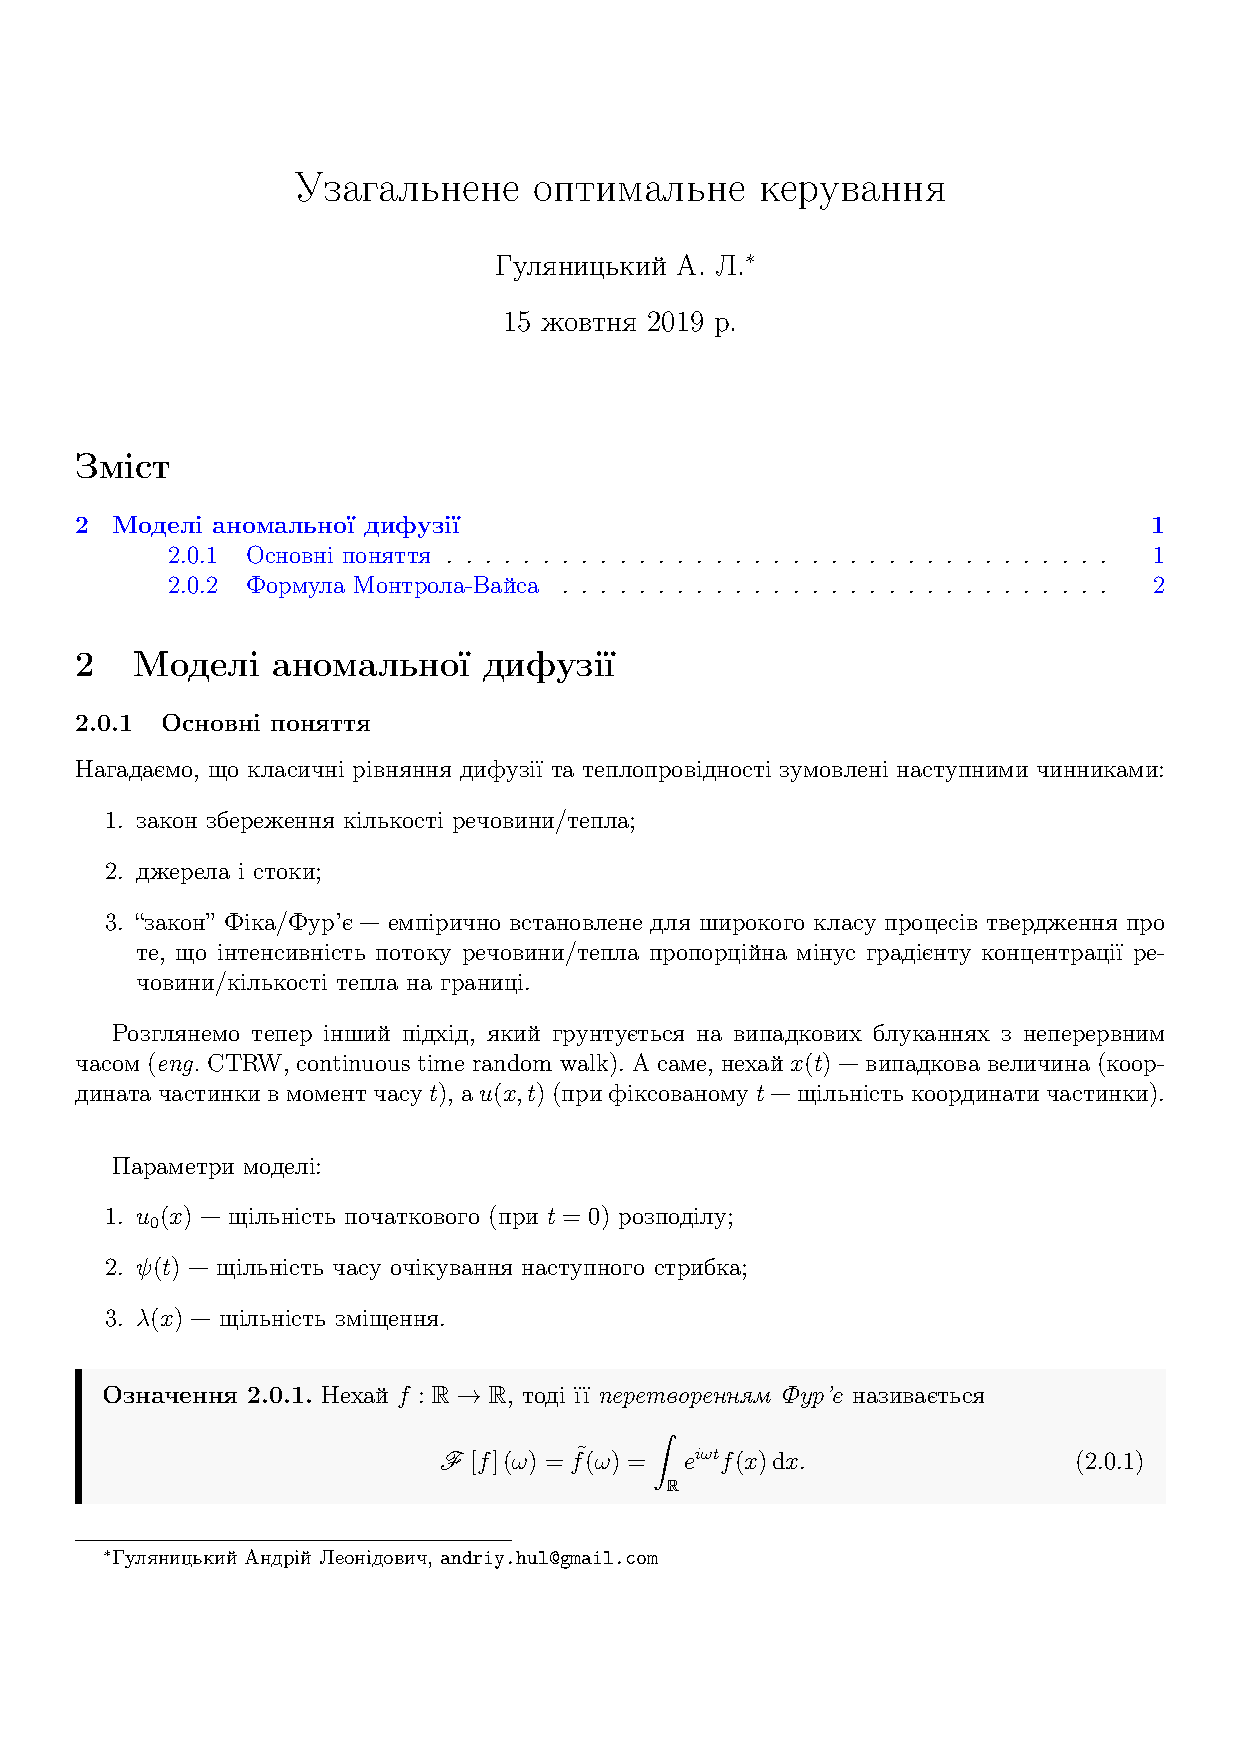
\includegraphics[width=.5\textwidth]{{img/05/05}.mps}
        \end{figure}
        
        \item Інший варіант -- взяти апроксимацію
        \begin{equation}
            \label{eq:4.3.15}
            A_h y_h = y_{t, i}^j + y_{\bar x x, i}^{j + 1}
        \end{equation}

        Тоді $\text{Ш}(x) = \{(x_{i - 1}, t_{j + 1}), (x_i, t_{j + 1}), (x_{i + 1}, t_{j + 1}), (x_i, t_j)\}$:
        \begin{figure}[H]
            \centering
            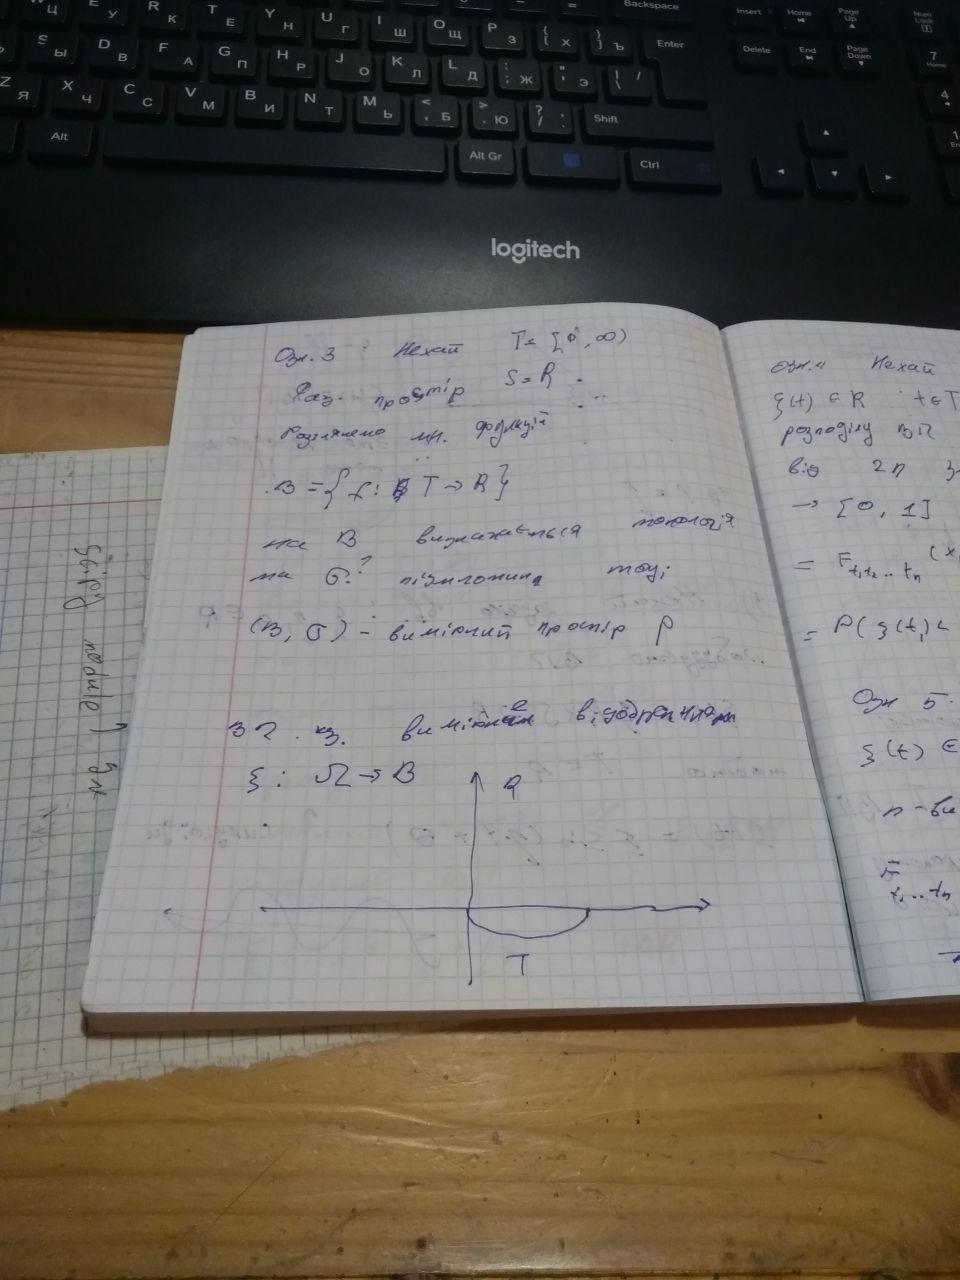
\includegraphics[width=.5\textwidth]{{img/05/06}.mps}
        \end{figure}
    \end{enumerate}
\end{solution}
